% vim: set tw=78 tabstop=4 shiftwidth=4 aw ai:

\chapter{Peer-to-Peer Systems and Protocols}
\label{chapter:p2p-systems}

Peer-to-Peer (P2P) has become a "buzzword" in the early 21st century and is
now one of the most common technology used. Although until 2000, the most
common paradigm in Internet was client-server, once the emergence of Napster,
Peer-to-Peer technology has become one of the most used and controversial
technologies.

With a total of 60 million users in 2001 and many terabytes of music shared,
Napster became the center of public attention and the promoter of P2P
technology. Soon after that, a series of Peer-to-Peer solutions led to a new
way of sharing information, files, knowledge and data (JXTA, Gnutella,
BitTorrent, DirectConnect, Jabber).

In literal translation, "peer-to-peer" means communication between equals,
between two autonomous entities and independent of each other. In principle,
a "Peer-to-Peer" system is a decentralized system: each node in the network
has the same role as any other node. The opposite is a client-server system,
which is centralized on the server. An immediate advantage of Peer-to-Peer
architecture is scalability and fault tolerance.

\begin{figure}
  \centering
  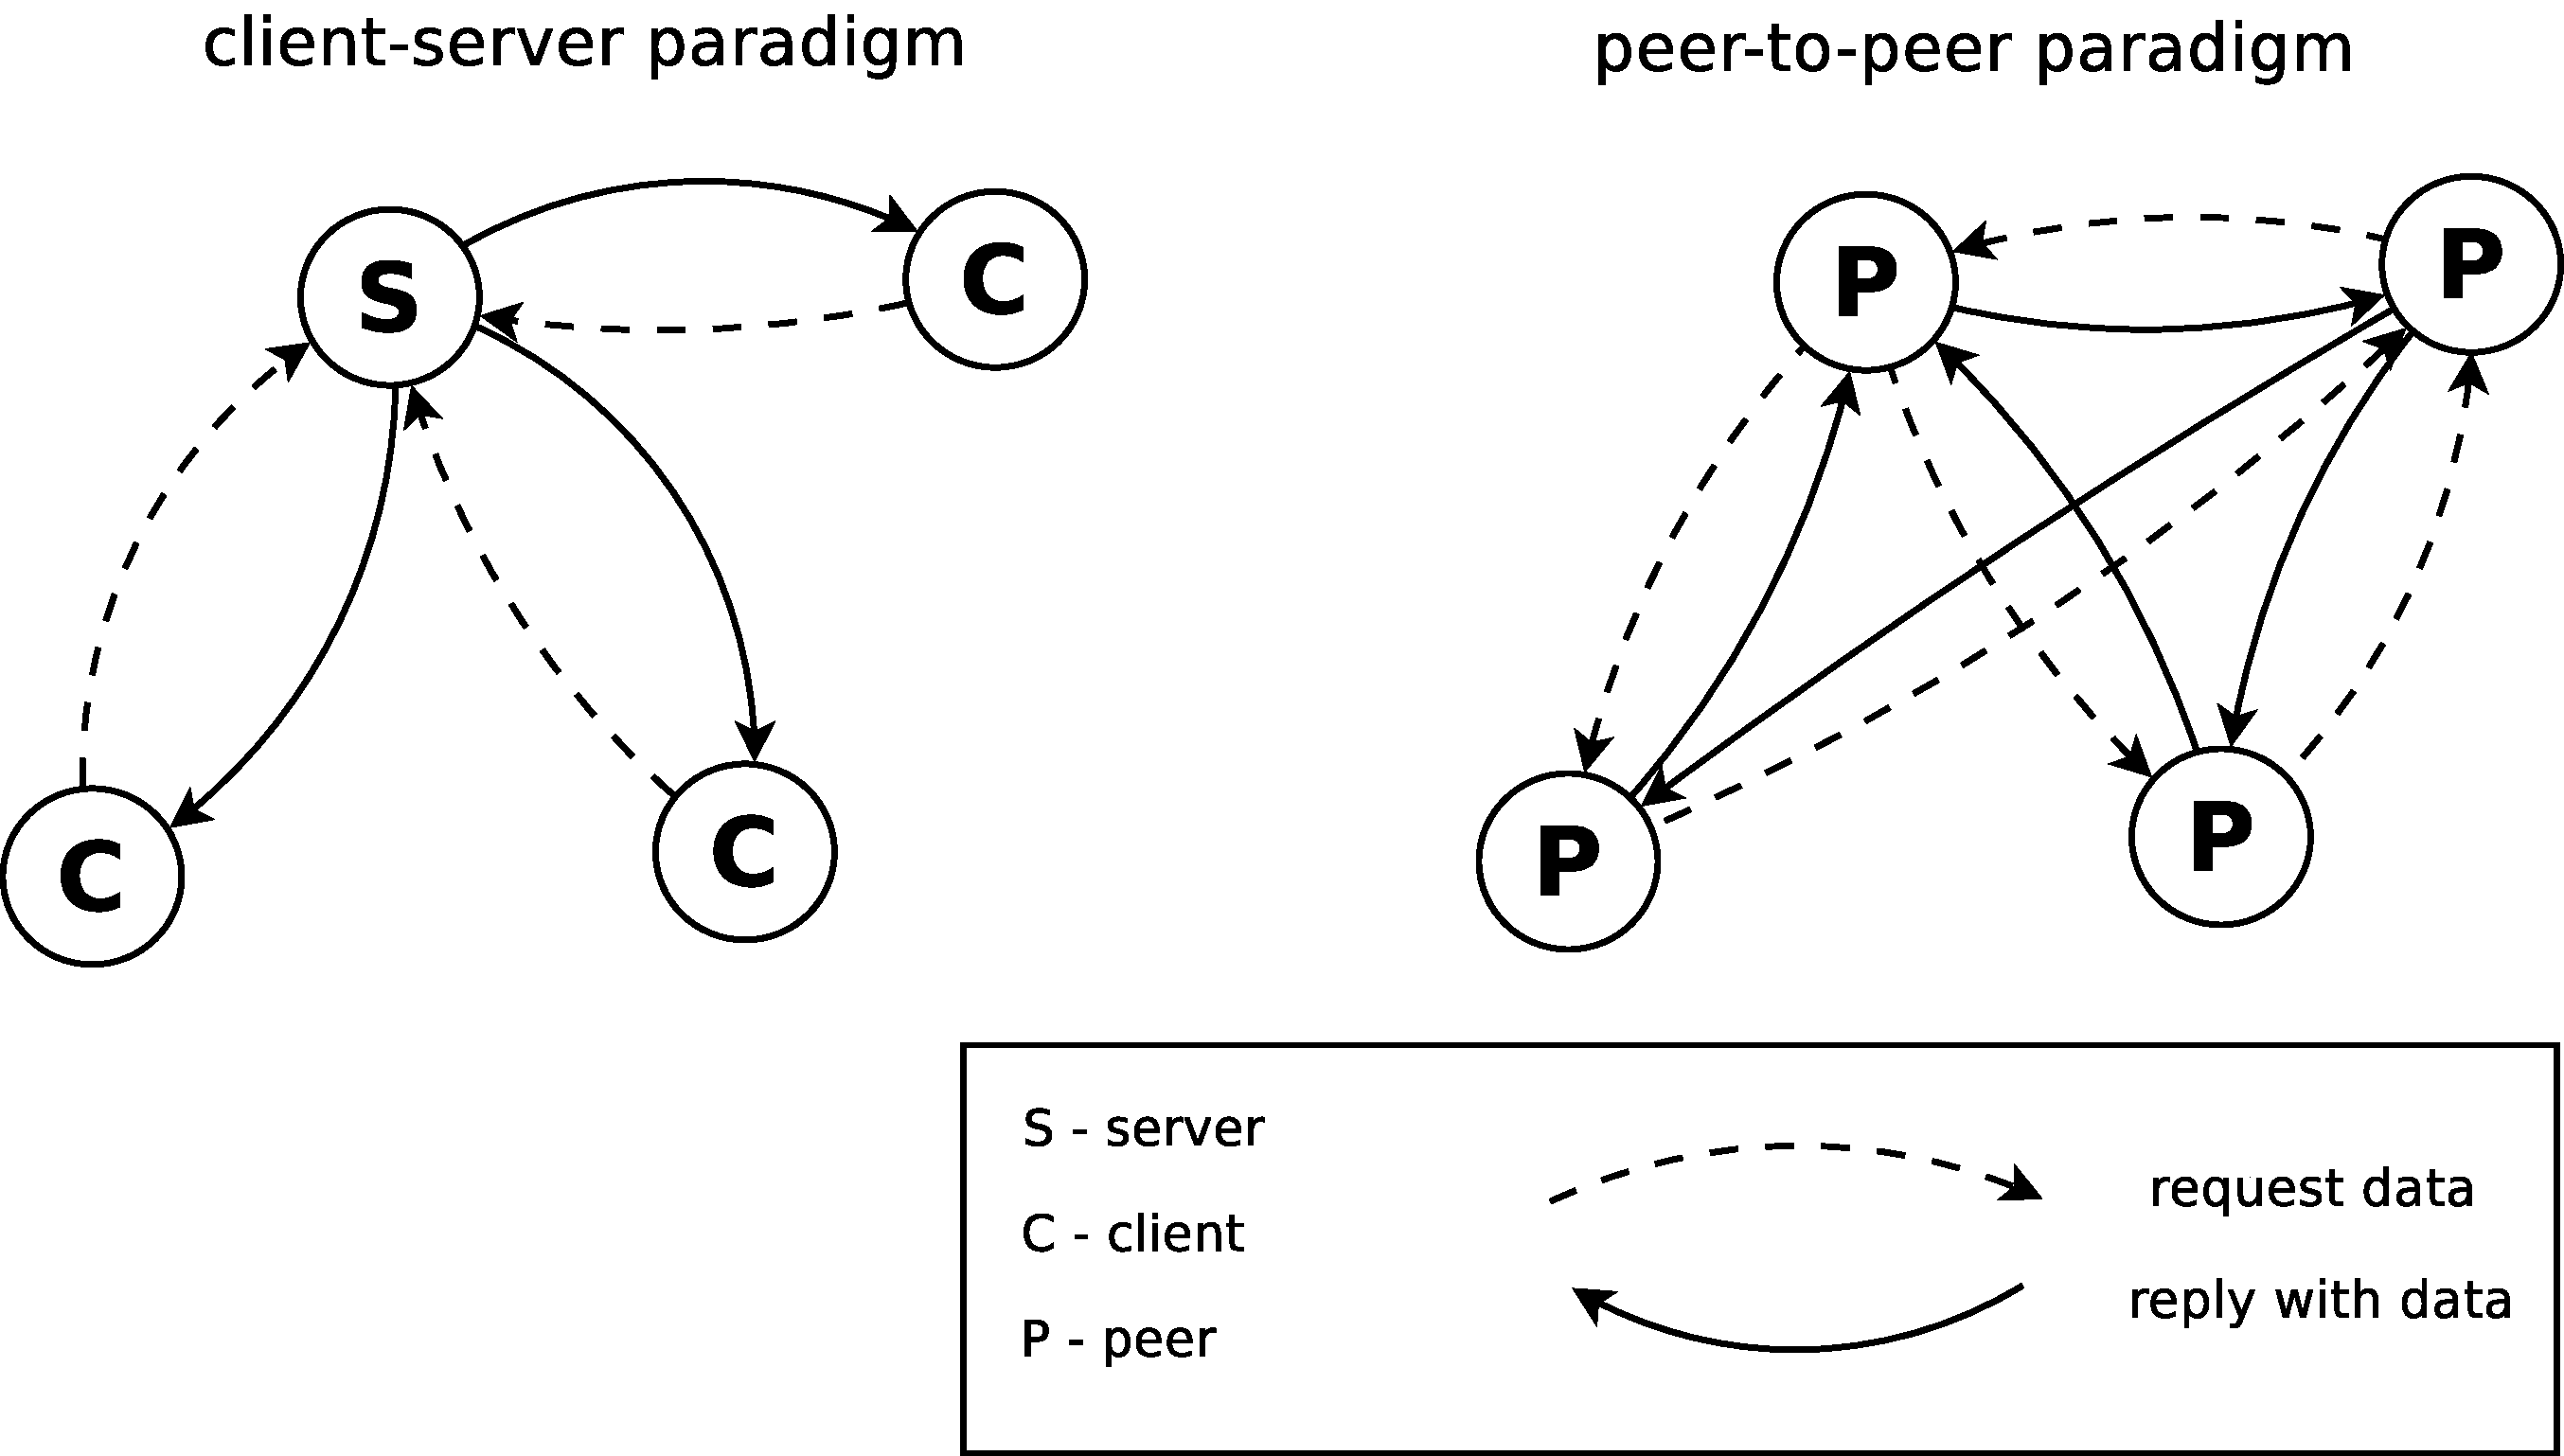
\includegraphics[width=0.7\textwidth]{src/img/p2p-systems/client-server-vs-p2p}
  \caption{Client-Server versus Peer-to-Peer}
  \label{fig:p2p-systems:client-server-vs-p2p}
\end{figure}

To consider a system "peer-to-peer", it must respond affirmatively to the
following questions:
\begin{itemize}
  \item It deals with variable connectivity and temporary addresses as a matter
 of course?
  \item It provides autonomous visibility for nodes at the edge of network?
\end{itemize}

In addition,there is a third default condition, which states that communication
between nodes must exists for the system to work.

It is noticeable that these conditions don't require a decentralized
architecture as peer-to-peer systems are usually charged. These conditions
require that each network node is an independent player and is not mandatory
for the system to work.

The Internet is a shared resource, a reservoir of information and a cooperative
network built with millions of nodes worldwide. As from 90s, the Internet has
experienced an explosive growth which generated an acute demand for one of the
basic network resources: bandwidth. The Firewall arose from the need of
supporting a variety of applications with constraints regarding security.

However, in 2000 everything changed, or, better said, returned to initial
condition. Passive elements have become active elements. Through sharing of
music files (via Napster) and through a larger movement (called peer-to-peer),
millions of users connected to the Internet have begun to use their systems for
more than reading e-mails and browsing. Systems connected through the Internet
could form groups and collaborate to meet various needs.

\section{Evolution of the Internet}
\label{sec:p2p-systems:evolution-internet}

\subsection{Early Internet (1969-1995)}

In the ARPA project, the Internet was originally designed as a peer-to-peer
system. The first few nodes of ARPANET were nod connected in a client-server
relationship, but in a relationship of equality. However, the Internet at that
time was much more open and free than the Internet these days. Firewalls were
unknown and any pair of systems could send packets to each other.

First important applications of the Internet were electronic mail (e-mail), FTP
and telnet. Although applications followed client-server paradigm, utilization
cases were symmetrical. Each station could use telnet or FTP to connect to any
other station.

Symmetry of the Internet has allowed the existence of complex peer-to-peer
systems such as Usenet or DNS. In subsequent years, the Internet has become
increasingly restricted only to applications that used client-server paradigm.
However, with the emergence of peer-to-peer applications, the trend of the
Internet is to return to the original design.

\subsection{Internet Expansion (1995-1999)}

In 1994 the Internet changed. Millions of people have started using it. Where
hitherto the Internet was an object of study for computer networks scientists,
now ordinary people have become interested to send messages, view Web pages or
to purchase various articles.

Changing the Internet into a mass cultural phenomenon had an tremendous impact
on networking architecture. The changes are reflected in sharing collaboration
on the Internet and increasingly often usage of firewalls.

The spectacular growth of the Internet, the firewalls usage and NAT led to the
proliferation of client-server paradigm of the Internet. The Web browser was a
application based on a simple client-server protocol: a client requests a
page, the server provides it and after the connection is closed. The client
systems don't have to have a permanent address or a well-known address.

The Internet boom-period was characterized by the break of collaborative mode
which was originally designed with. Firewalls, dynamic IP addresses, NAT usage
are technologies that have led to a strict division of the Internet between
servers and clients. The directly result is that many stations are harder
to be accessed through the Internet. Peer-to-peer applications such as
messaging or file-sharing should work hard to pass there limitations.

\subsection{Rebirth of the Peer-to-Peer Paradigm}

Since 2000 (Napster), peer-to-peer applications have become more common and
widely used. Peer-to-peer applications allow easy publication of information
and designing of decentralized applications, which is simultaneously a challenge
and an opportunity.

In this case, peer-to-peer model is closely linked with the idea of
decentralization. In a fully decentralized system, each node is an equal
participant without having any special role. DNS is a peer-to-peer protocol
that has the implicit idea of hierarchy. Many other peer-to-peer systems have
a semi-centralized organization with some nodes having special roles.

However, peer-to-peer applications encounter server problems in current
architecture of the Internet: firewalls and NAT makes more difficult creating
connections between stations. Asymmetric bandwidth prevents users from
efficiently serve files from their computers.

Beyond technical problems, peer-to-peer applications face social problems.
Sharing files in a peer-to-peer system must take into account free-riders.
Free-riders are those who use others shared files without sharing anything. For
this, there must be a form of accounting effort for each customer.

Also, since the launch of Napster, peer-to-peer applications have attracted
many issues related to sharing copyrighted materials. Here we refer to audio,
video, electronic documentation, etc.

\section{The Peer-to-Peer Paradigm}
\label{sec:p2p-systems:paragigm}

\subsection{Features and Models of Peer-to-Peer Systems}

As mentioned previously, the characteristics of P2P networks are sharing and
distribution of resources, decentralization and autonomy.

Sharing and distribution of resources refers to the operation each node of the
peer-to-peer network has. A node can function as a server or as a client and
can act as a provider and as a consumer of resources and services (information,
files, bandwidth, storage, processor cycles). These nodes are also called
???servanți???.

Decentralization refers to the absence of a central coordinating authority for
organizing network or for resources usage and communication between nodes.
Communication takes place directly between nodes. Frequently, there is a
distinction between pure P2P networks and hybrid networks. In hybrid P2P
networks, certain functions (such as indexing and authentication) are allocated
to a subset of nodes that have coordinating role.

Autonomy means that each node independently decides what resources gives to
other nodes.

The lower cost for processor cycles, bandwidth and storage space combined with
the growth of the Internet have created new areas for applying P2P networks.
This has led to explosive growth of P2P applications and to discussions about
limitations, performance and economic, social and legal topics.
Figure~\ref{fig:p2p-systems:p2p-levels} shows a model based on P2P
infrastructures, applications and communities.

\begin{figure}
  \centering
  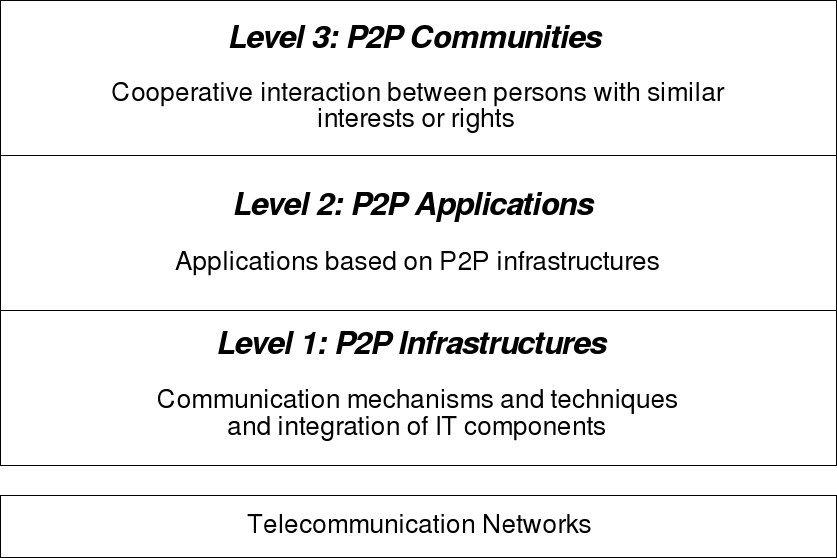
\includegraphics[width=0.7\textwidth]{src/img/p2p-systems/p2p-levels}
  \caption{Peer-to-Peer Levels}
  \label{fig:p2p-systems:p2p-levels}
\end{figure}

P2P infrastructures are positioned over existing communication networks and
acts as a foundation for other levels. P2P infrastructures provide
communication, integration and translation between various IT components. It
also provides search services, communication and sharing between network
nodes and initiation of security processes such as authentication and
authorization.

Level 2 is represented by P2P applications that use P2P infrastructure
services. Applications are used to allow communication and collaboration
between different entities in the absence of a central controller.

Level 3 focuses on the social networking phenomenon; in particular, on building
communities and their dynamics.

\subsection{P2P Resource Management}

In specialized literature, P2P applications are often classified in categories
such as: instant messaging, file sharing, grid computing and collaboration.
This classification has been developed over time and fails to make clear
distinctions between different applications. Today, there are many situations
where many categories can be considered equivalent. For these reasons, another
classification could take into account issues regarding resources usage in P2P
systems.

Thus, there is a classification of P2P systems regarding available resources.

\subsubsection{Data}

Information is used in collaborative spaces in the form of sharing or exchanging
information and document management. Information about the presence of nodes in
P2P systems is fundamental for the organization of a P2P system and for
knowledge of resources they make available. Presence information is useful to
knowledge of free CPU cycles on a computer system that can be used in a grid
application.

DMS (Document Management Systems) are storage spaces that enables shared storage,
management and use of data. Formation of collaborative groups for document
management is a result of information-sharing applications (P2P groupware). In
client-server groupware systems, a workspace for the information management
is needed. A P2P system can avoid all tasks related to the administration
of that workspace.

\subsubsection{Files}

Sharing files is the most common form of P2P applications. 70\% of the Internet
traffic can be attributed to file exchange (mostly media files). One of the main
problems of P2P systems (and file sharing applications) is localizing resources.
In the context of file sharing systems have been developed three algorithms:
flood model, centralized directory model and conveyance documents model. These
models are best illustrated by prominent implementations like Gnutella, Napster
and Freenet.

\subsubsection{Bandwidth}

With increasing demand for transmission capacity of networks, mainly due to
increasing multimedia transfer, effective use of bandwidth becomes more
important. Usually, centralized approach where files are kept on the server
goes to occurrence of a bottleneck in the system when simultaneous requests
arrive from multiple clients.

In these situations, using a P2P systems have two advantages: increasing load
balancing using unexploited transmission routes; usage of shared bandwidth that
allows accelerate download and transport of large files simultaneously
requested by various entities. Generally, there files are divides into small
blocks downloaded simultaneously from different nodes of the network.

\subsubsection{Storage}

Increasing connectivity and bandwidth availability allows alternative forms of
storage management that solves these problems and requires less administrative
effort. In P2P storage networks, only a portion of a desktop PC space will be
used. A P2P storage network is a cluster of computers based on networks sharing
existing storage. When a file is stored in the network, a unique identification
number (obtained by applying a hash function on the content of file name) is
assigned. In addition, a number of copies of the file are also stored on the
network.

\subsubsection{CPU Cycles}

Recognising that computer networks have unused computing power, led in trusting
P2P application to use that power. Using P2P application for collecting CPU
cycles can achieve a computing power that can be supplied very difficult even
with most expensive supercomputers. This type of approach of using coordinated
resources of distributed computing that extend beyond a simple institution
falls under the auspices of the domain "grid computing".

One of the most common example of grid projects in the context of P2P networks
if SETI@home. SETI@home is a scientific initiative launched by University of
California, Berkeley, in order to discover radio signals from extraterrestrial
intelligence. For this purpose, a radio telescope from Puerto Rico records a
portion of the electromagnetic spectrum space. Data are transmitted to the
central server based in California. Instead of analyzing data using
supercomputers, the server divides the information into small units and sends
them for processing to millions of computers volunteered to participate in this
project.

\subsection{P2P Topologies for File Sharing}

P2P networks topology refers to: how nodes are connected, the existence of
specialized nodes, transfer mode for shared file or meta-information. In terms
of network topology, P2P systems have two main characteristics:

\begin{itemize}
  \item scalability: there is no technical or algorithmic limitation for the
  system size; system complexity must be relatively constant compared to the
  number of nodes in the system
  \item reliability: the lack of functioning of a given node will not affect
  the whole system (if possibly, neither other nodes)
\end{itemize}

P2P systems can be grouped into two categories: pute P2P systems and hybrid P2P.
Pure P2P systems (such as Gnutella or Freenet) have no central server. Hybrid
P2P model (such as Napster, eDonkey2000 or Groove) uses a central server to
obtain meta-information or to verify credentials. In a hybrid system, nodes
always contact a central server before directly contact other nodes.

All P2P topologies, regardless of differences, have one common feature: all
information transfers between nodes are achieved through direct connection
between knots. However, the control of the process can be implemented in several
ways. As a result, P2P networks can be classified into four major categories:
centralized, decentralized, hierarchical and ring. Although these topologies
can exist by itself (independent), distributed systems have more complex
topologies by combining some basic systems for creating what is called hybrid
system.

\subsubsection{Centralized}

Centralized topology concept is based on the traditional client-server paradigm.
There must be a central server used to control files and databases with users
nodes that enter the system. The client contacts the server to inform about his
current IP address and the file names he want to share. This is performed
whenever the application is launched. Information collected from nodes will then
be used by the server to create a centralized dynamic database that maps file
names with sets of IP addresses.

\begin{figure}
  \centering
  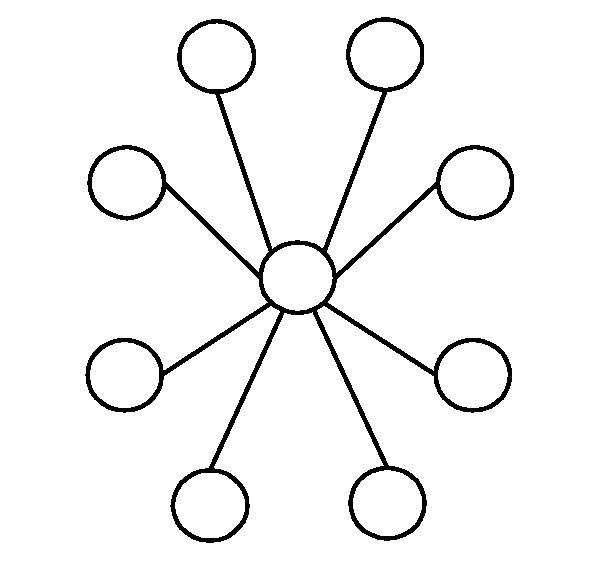
\includegraphics[width=0.4\textwidth]{src/img/p2p-systems/centralized}
  \caption{Centralized Topology}
  \label{fig:p2p-systems:centralized}
\end{figure}

All search requests are submitted to the server which will consult his local
database. If a match occurs, it creates a direct link to the node sharing the
file and run the transfer. In no situation the shared file will be present on
the server.

\subsubsection{Ring}

The most important disadvantage of centralized topology is that the central
server can become a bottleneck in the system (if load material) and a critical
point in case of failure. In these contexts, ring topology has appeared.

\begin{figure}
  \centering
  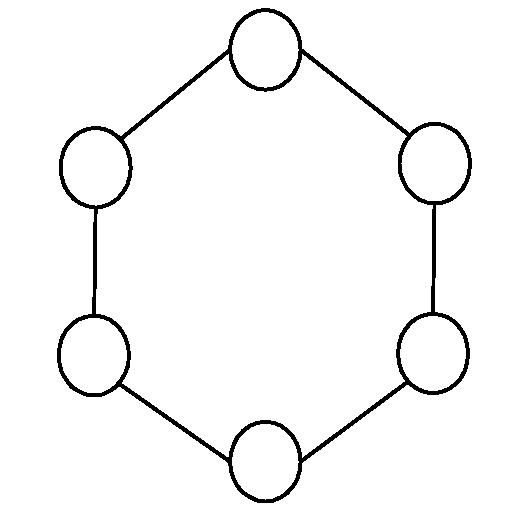
\includegraphics[width=0.4\textwidth]{src/img/p2p-systems/ring}
  \caption{Ring Topology}
  \label{fig:p2p-systems:ring}
\end{figure}

Ring topology is made of a cluster of systems that are arranged in a ring shape
to act as a distributed server. This cluster provides the best possible load
balancing for higher availability. This topology is commonly used when systems
are relatively close topological and, quite likely, held by a single
organization where anonymity is not so important.

\subsubsection{Hierarchical}

Hierarchical topology exist from the beginning of human civilization. The most
famous example of a hierarchical system in the Internet is DNS (Domain Name
System). Authority delegates from the root name servers to the registered name
server. The topology is suitable for systems that requires a government form
involving delegation of rights or authority. Another example is the certification
authority (CA) that certifies the validity of an entry in the Internet.

\begin{figure}
  \centering
  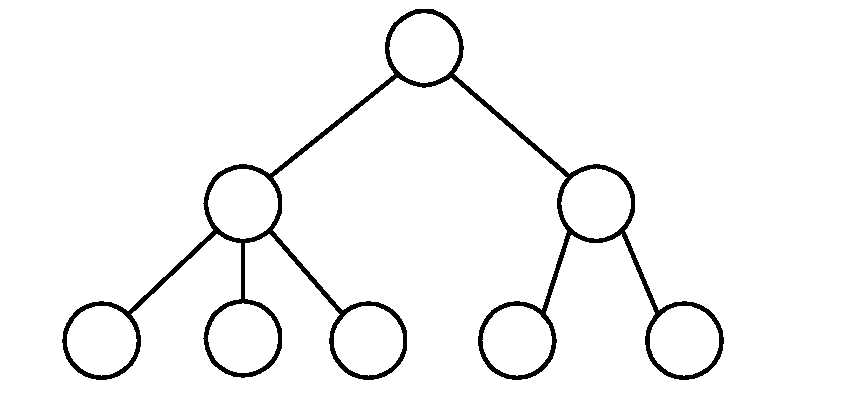
\includegraphics[width=0.4\textwidth]{src/img/p2p-systems/hierarchical}
  \caption{Hierarchical Topology}
  \label{fig:p2p-systems:hierarchical}
\end{figure}

\subsubsection{Fully Decentralized}

In a pure P2P architecture, there are no centralized servers. All nodes are
equal resulting in obtaining a flat topology, unstructured. To join the network,
a node should contact a bootstrap node (node which is always online). This will
provide to the new node, IP addresses of one or more nodes already in the
network, making it officially part of the dynamic network. However, each node
will have only information about its neighbors - nodes which are directly
connected with it.

\begin{figure}
  \centering
  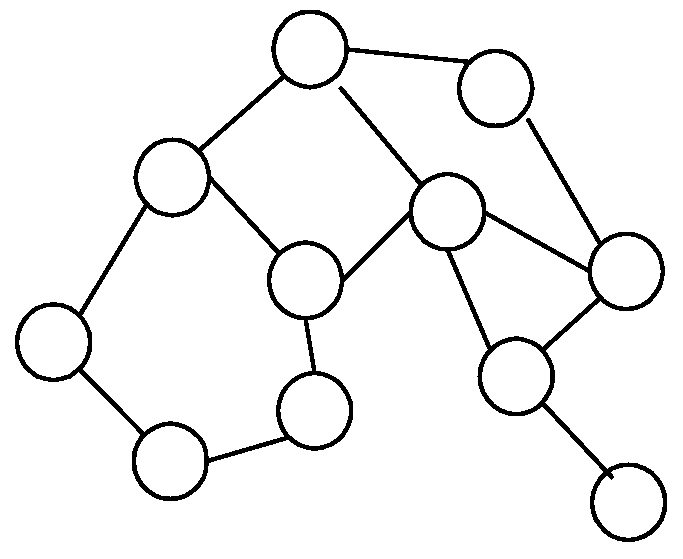
\includegraphics[width=0.4\textwidth]{src/img/p2p-systems/decentralized}
  \caption{Fully Decentralized Topology}
  \label{fig:p2p-systems:decentralized}
\end{figure}

Since there are no control server for searching, file requests are sent in the
form of floods through the network. As a result, flooding additional loads the
network bandwidth.

\subsubsection{Hybrid}

Today, P2P networks combine many of the basic topologies from above. They are
also called hybrid architectures. In such systems, nodes will often play several
roles.

\subsubsection{Centralized Ring}

This hybrid topology is very common for Web hosting systems. As mentioned
previously, Web servers typically have a ring of servers specialized in load
balancing and defects tolerance. Thus, servers are arranged in a ring topology.
Clients are connected to ring topology using a centralized topology.

\begin{figure}
  \centering
  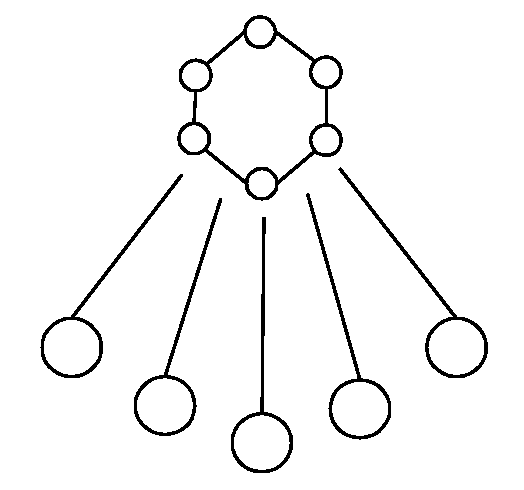
\includegraphics[width=0.4\textwidth]{src/img/p2p-systems/centralized-ring}
  \caption{Centralized Ring Topology}
  \label{fig:p2p-systems:centralized-ring}
\end{figure}

\subsubsection{Centralized-Centralized}

It can happen often that one server of a network to be a client in a larger
network. This hybrid topology is very common in organizations that provides
Web services.

\begin{figure}
  \centering
  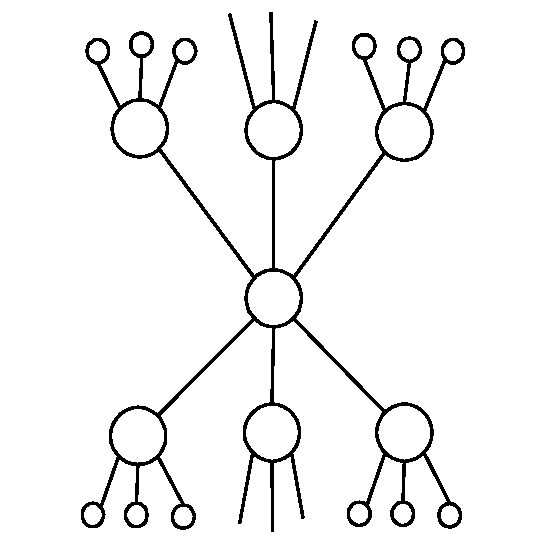
\includegraphics[width=0.4\textwidth]{src/img/p2p-systems/centralized-centralized}
  \caption{Centralized-Centralized Topology}
  \label{fig:p2p-systems:centralized-centralized}
\end{figure}

\subsubsection{Centralized-Decentralized}

In this topology, some nodes function as group leaders (usually called
Super-Nodes). Super-Nodes provides server tasks only in a subset of nodes.
Super-Nodes are connected in a decentralized manner.

\begin{figure}
  \centering
  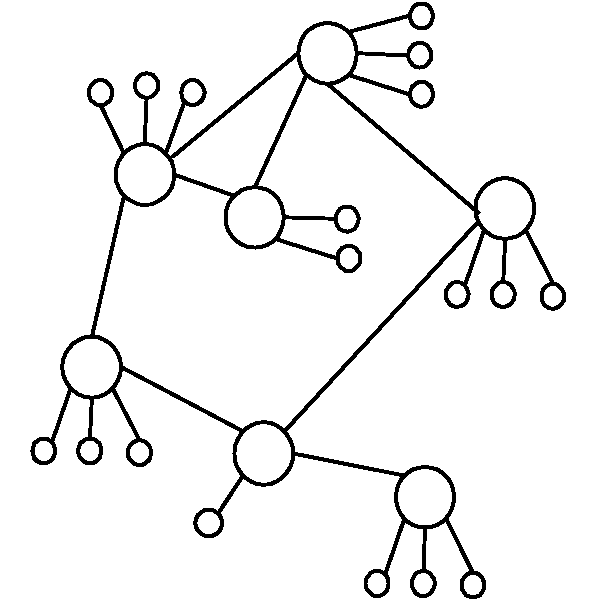
\includegraphics[width=0.4\textwidth]{src/img/p2p-systems/centralized-decentralized}
  \caption{Centralized-Decentralized Topology}
  \label{fig:p2p-systems:centralized-decentralized}
\end{figure}

As in a centralized topology, Super-Nodes maintain a database that maps IP
addresses with files. Super-Nodes database maintains information only about
the group knots. A sample of application that uses such P2P topology is
FastTrack. Another example of such a topology is the e-mail from the Internet.

\section{Peer-to-Peer Systems in the Internet}
\label{sec:p2p-systems:p2p-internet}

\subsection{Napster}

Napster was the first successful example of a peer-to-peer system. Napster was
permanently closed in June 2001 and marked the end of an outstanding era, with
65 million users in only 20 months. Napster  central control model was possible
due to focusing user approach.

Figure~\ref{fig:p2p-systems:napster} presents the essential architecture
components of Napster where communication is mediated by the server. Clients
are connecting to a well known "meta-server". The "Meta-server" associates a
server with reduced load from one of the clusters. In a cluster there are 5
servers and each one can control about 15.000 users.

\begin{figure}
  \centering
  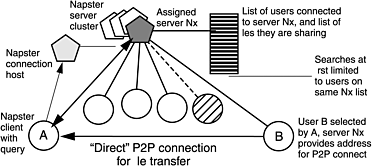
\includegraphics[width=0.7\textwidth]{src/img/p2p-systems/napster}
  \caption{Napster Architecture}
  \label{fig:p2p-systems:napster}
\end{figure}

The client register with the associated server, providing information about
its identity and shared files. Then, it receives information about other online
users and about available files. Users are anonymous to each other and local
directory structure is not directly questioned. The main interest is searching
for content and determine where can be download the resource from. Server's
directory is only used to translate between station identity, the desired
resource and the IP address necessary to initiate the connection.

Because network performance is essential, searches are constrained to a maximum
of 100 hits and maximum 15 seconds duration. Searches take place in the local
database maintained by the server, but, sometimes, can be passed to neighboring
servers within the same cluster.

Conceived originally as a system for sharing MP3 files, a whole culture of
clones and utilities appeared. However, this had disadvantages too. For example,
there are tools (like Wrapster) that could make other files look like MP3 files.
Other utilities (such as Napigator) allowed users connect to certain servers,
bypassing the "meta-server" arbitration phase.

However, no matter how much Napster has been redesigned, it still used a
centralize and compatible server. This meant a serious constraint for a network
based on this technology or on any of its clones. To change this limitation,
there were designed other protocols and architectures, serverless, in the style
of Gnutella.

\subsection{Gnutella}

Initially, Gnutella was the name of a prototype client developed in just a few
weeks in March 2000 by the same team that created WinAmp. At its beta version
launching, almost everyone saw Gnutella as a competitor for Napster, designed
to overcome many of its limitations. However, AOL, who just bought Nullsoft,
decided to immediately stop working on the client. Everything would have ended
here if hadn't been Bryan Mayland who managed to deduce Gnutella protocol and
published its specifications on the Internet. Soon began the development of
Gnutella open-source project.

These days, Gnutella is a generic term with various meanings: the protocol, the
open-source technology and the Internet network used. There are several clients
for Gnutella protocol and, although most of them focuses of sharing and
searching files, they can achieve many operations.

Today, Gnutella is mainly a file sharing network that allows arbitrary types of
files. There is no central server and therefore there is no point of failure.
Public or private networks are defined only by clients who are currently in
communication with each other. Each user can build a local map of the network
capturing messages from the other clients. There can be more networks, depending
on how clients are configured to interconnect.

The lack of a central control point in Gnutella means that the legal
responsibility for file transfers remain in user hands. Depending on the point
of view, it may be a good or a bad thing. On gNET can be found illegal copies
of almost everything one can think of.

There is no standard client, but there are several clients built on Gnutella
protocol. This clients can communicate with each other, but developers have
liberty for functionalities and extensions implementation. Gnutella
specifications and most of the clients are open-source. However, there are
also proprietary implementations.

Authentication in a network like Gnutella is similar with a group of people
looking into different directions. A user only communicate with immediate
neighbors and through there neighbors can communicate with the others. In each
sessions, there is a different selection of people and resources.

In principle, a node can connect to any node from its neighborhood. But just
like in real life, some nodes may be too busy to talk and will not provide
attention. Other nodes will completely ignore the connection request. Other
nodes will change a few word and will move on. Eventually, it will reach a node
they can establish a long-term contact and to which they can send requests and
results. Nodes appear and disappear continuously and local configuration requests
will change constantly so that over time, a node will connect to multiple nodes.

\begin{figure}
  \centering
  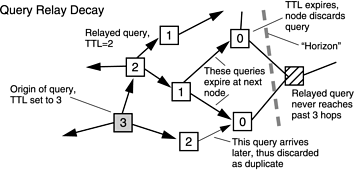
\includegraphics[width=0.7\textwidth]{src/img/p2p-systems/gnutella}
  \caption{Gnutella Architecture}
  \label{fig:p2p-systems:gnutella}
\end{figure}

Atomistic P2P networks such as Gnutella are very dynamic and don't have central
addresses lists. From a pragmatic point of view, a list of bootstrap for initial
discovery is needed.

The "horizon" effect relates to the inherent virtual segmentation of the
network, ... Efectul de "orizont" ține de segmentarea virtuală inerentă
a rețelei, o decizie de proiectare care limitează contorul de noduri la
circa 15.000 pe gNet, noduri vizibile de la un alt nod. ... Nodes continue to
enter and leave the netowrk thus influencing nodes that can be reached. The
main reason for the occurrence of "horizon" effect is that messages have a
counter time-to-live (TTL). Typically, TTL is set between 5 and 7 and is
decremented by each node through which the message passes. Another counter
monitors the number of hops. TTL's values and the number of connected nodes,
together with bandwidth and capacity of a node, combine to determine performance
and network stability. Some clients allow the user to manually adjust the TTL
and the number of active nodes, thus succeeding in expanding horizon.

În Table~\ref{tab:p2p-systems:gnutella-horizon} we can see horizon progress
(number of nodes that can be reached) reported to TTL value and the number of
nodes connections:

\begin{table}[htb]
  \centering
  \caption{Gnutella Horizon Evolution (number of reachable nodes)}
  \label{tab:p2p-systems:gnutella-horizon}
  \begin{tabular}{@{}lrrrrrr@{}}
    \toprule
      & \textbf{TTL=2} & \textbf{TTL=3} & \textbf{TTL=4} & \textbf{TTL=5} &
      \textbf{TTL=6} & \textbf{TTL=7} \\
    \midrule
      \textbf{N=2} & 4 & 6 & 8 & 10 & 12 & 14 \\
      \textbf{N=3} & 9 & 21 & 45 & 93 & 189 & 381 \\
      \textbf{N=4} & 16 & 52 & 160 & 484 & 1456 & 4372 \\
      \textbf{N=5} & 25 & 105 & 425 & 1705 & 6825 & 27305 \\
      \textbf{N=6} & 36 & 186 & 936 & 4686 & 23436 & 117186 \\
      \textbf{N=7} & 49 & 301 & 1813 & 10885 & 65317 & 391909 \\
      \textbf{N=8} & 64 & 456 & 3200 & 22408 & 156864 & 1098056 \\
    \bottomrule
  \end{tabular}
\end{table}

\subsubsection{The Gnutella Protocol}

Gnutella protocol is highly correlated with HTTP protocol. All nodes have equal
rights and each node is simultaneously client and server. Gnutella is
open-source and is a simple protocol, specifications being present in various
locations on the Web.

Gnutella protocol defines only five descriptors (message headers) to implement
network functionality. Each message descriptor is defined by a message header
whose components are shown in the table below. The header is simple, containing
only 5 files.

\subsubsection{Connection and Discovery}

Gnutella clients communicate using default port 6346 and HTTP/1.0 that gives a
mini-browser/mini-server functionality. Network connections are established by
sending the message below through a TCP connection:

\begin{verbatim}
GNUTELLA CONNECT/<protocol version string>\n\n
\end{verbatim}

A node who wishes to accept the connection will respond with:
\begin{verbatim}
GNUTELLA OK\n\n
\end{verbatim}

Any other response indicated that the node does not want to accept that
connection.

A customer may choose to reject a connection for a variety of reasons. A client
may choose to maintain only existing connections and reject any other requests.
There may be limitations of slot connections or a service could not operate on
the protocol used and reject the connection.

Nodes already connected to the network can map active nodes addresses through
ping-pong messages from other nodes because Gnutella protocol doesn't specify
an initial method for discovery before connection establishment. At the
beginning, quasi-permanent addresses are distributed through other channels
and new users introduce them in clients until a new connection is established.
Nowadays, node addresses are bought automatically through caching services
implemented on some "permanent" network nodes.

With the above configuration, clients can automatically maintain local lists
for downloads and can use them later from the local cache. Once connected to an
active node, clients can map other nodes by sending ping-pong messages. As a
result, clients can establish new connections. Below is presented a map of
connections, limited to a hop count of 4.

Ping-pong messages are a significant portion of traffic in a P2P network,
totaling about two-thirds or three-quarters of all messages through any
connection. Therefore, Gnutella protocol recommends to minimize the number
and frequency of ping packets transmitted by any client.

\subsubsection{Search}

Search is fundamental for Gnutella protocol and is implemented with Query
messages. Usual method of broadcasting requests means that every service
can obtain, verify its validity, make a cache entry of the identifier and
forward the request to other existing connections. After that, the application
provides a search on its own content.

In addition to the searched string, the description starts with a field that
specifies the minimum transfer rate of response. This is how is indicated for
nodes with lower transfer rates not to bother to respond. However, they will
continue to forward the request. Nodes that find a matching string respond
with a Query Hit message. The message contains information about the node and
how connectivity can be made. Query Hit messages are sent back to the network
with the same identifier as the request. This allows the initial client to
identify and associate received Query Hit messages with initial Query messages.

Here is an example of transfer request initiated by client:

\begin{verbatim}
GET /get/<File Index>/<File Name>/ HTTP/1.0\r\n
Connection: Keep-Alive\r\n
Range: bytes=0-\r\n
User-Agent: <Agent Identifier>\r\n
\r\n
\end{verbatim}

If everything goes well, the service will respond with a confirmation header:

\begin{verbatim}
HTTP 200 OK\r\n  Server: <Agent Identifier>\r\n
Content-type: application/binary\r\n
Content-length: 4356789\r\n
\r\n
\end{verbatim}

An appropriate response allows the node performing the request to start
downloading the file. The user will determine whether the bandwidth and
reliability of the destination node are satisfactory and, if it is, will start
the transfer.

\subsubsection{Transfer}

Although file transfer takes place directly between the two ends and doesn't
load the rest of the network, bandwidth is shared with other transfers. In
addition, bandwidth can be reduced by the client and uploads limited to a
certain value, despite of a large bandwidth. It is not uncommon for a transfer
rate to be very high initially and fall to unacceptable levels in time.

Range parameter in the message involves the ability to resume, from a given
offset, interrupted transfer. The ability to resume transfers is essential in
rapidly changing networks where each node may disconnect in its own will.

Today, clients support for different file segments from different nodes.
Parallel transfers from different offsets improves efficiency and reliability
and is often a technique implemented in advanced protocols.

However, the problems consists in correct identification of sources as copies
of the same file. A simple method is to move different parts of fragments with
a small value and verify the value of that displacement. In transferring
resumption, receiving client must remember the address of the associated node.
Otherwise, it would be forced to carry out a new search that can lead to
lack of fragment from the file.

\subsubsection{Scalability}

A Gnutella network exemplifies the advantages and disadvantages of an atomistic
P2P architecture, especially in the context of what is called "Transient Web".
Just as we have seen in the growth of the Internet about constrains of
the scalability and basic architecture.

Installing and using Gnutella in an internal network is not difficult.
Administrative tasks are limited to installing a list of supported nodes in the
clients. There are clients that provides options for creating such a special
type of "subnet".  Creating a limited network is not a problem. The main risk
of this context is whether a node should connect to a node not mentioned in the
predetermined list. Such a design would make the entire list of nodes accessible
from the outside. It only takes one client to suppress a "closed network" in the
absence of filtering measures for preventing such type of connections.

Solutions for a better security is introduced as technology matures. Examples
are automatic reliable systems and control of reputation.

\subsubsection{Trust and Reputation}

P2P basic implementations are usually open and have no form of management of
trust. Any computer that uses a compatible protocol and wants to connect to the
network is automatically accepted. However, total opening means that the network
is also opened for malware intrusion. Known attack methods are ping flooding,
request flooding, false found messages, denial of service attacks on discovered
nodes.

All clients can enable configurations to block connections based on specified
criteria, but the default behavior is not filtering anything. However, the
initial opening is changing and more and more clients begin to reconfigure the
default specifications with configurations less permissive. Typical filters
include closing connections with nodes that don't share content or have too few
connections and, additionally, specifying IP addresses for blocking.

There is a trend, lately, of increasingly importance to implement more
sophisticated features, which is visible in the innovative current
implementations. New forms of management P2P applications connectivity include
various forms of controlling trust and reputation, digital signatures and
encryption. The desire is that networks become more reliable and robust without
additional security measures. However, P2P developers also want to avoid central
administration and filtering, solutions characteristic to central-server
solution.

\subsection{FastTrack}

One of the latest and innovative  applications in peer-to-peer architectures
is FastTrack network. FastTrack arrived as a solution to Napster and Gnutella
problems. FastTrack architecture is hybrid by nature, which, as noted above, is
an intersection of two or more basic network topologies.  In FastTrack case,
we are talking about the intersection between centralized and decentralized
topologies.

FastTrack protocol is a proprietary architecture; using rights must be obtained
from the Sherman Networks company. Therefore, not so many things are known about
the current protocol. There were several attempts to understand FastTrack
protocol (reverse engineer). The most known is the giFT project, which was very
close to "break" the protocol. FastTrack reacted by changing the encryption
used so that is almost impossible deducting the protocol. However, the effort
was enough to define the operational mode of the protocol.

FastTrack uses two levels of control within its network, as shown in
Figure~\ref{fig:p2p-systems:fasttrack}. First level consists of clusters of
nodes that are connected to common Super-Nodes (common systems that offer
high-speed connections). As discussed previously, this type of connection is
similar to centralized topology. The second level consists of Super-Nodes
connected into a decentralized manner.

\begin{figure}
  \centering
  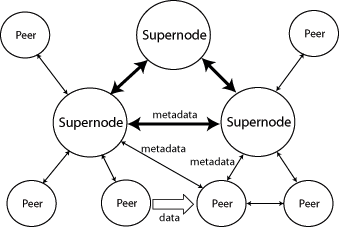
\includegraphics[width=0.5\textwidth]{src/img/p2p-systems/fasttrack}
  \caption{FastTrack Architecture}
  \label{fig:p2p-systems:fasttrack}
\end{figure}

The number of nodes defined as Super-Nodes can vary from tens to hundreds.
This happens because Super-Nodes are ordinary nodes that can enter or leave the
network when they want. As a result, the network is dynamic and in constantly
changing. To ensure constant availability, several nodes presence is required.
Such a node is called bootstrap node and must always be active (online). When
a FastTrack client (for example Kazaa) is running on a node, it will initially
contact the starting node. Next, the starting node will determine if that node
can be considered a Super-Node. If so, it will be given some (or perhaps all)
of th IP addresses of other Super-Nodes. If its classifies as a common node,
then starting node will respond by providing the IP address of one Super-Node.

Some clients (like Kazaa) use a method named reputation system. Reputation is
associated for each user and is reflected by the level of participation (a value
between 0 and 1000) in the network. The longer a user is connected, the higher
the level of participation is, so it will be favored in priority policies and
will receive the best services. This measure aims to encourage users to share
files and reduce the number of "passengers clients" on the network.

Resources are discovered through diffusion between Super-Nodes. When a node from
the second level makes a request, it's directed through the partner Super-Node
who will send the request to other Super-Nodes connected with it. Diffusion is
repeated until TTL's value reach 0. This provides to FastTrack client a greater
coverage and best search results. A disadvantage is the method of diffusion
consumption that can lead to a significant load of bandwidth between Super-Nodes.
However, this problem is not as serious like in the case of Gnutella and Kazaa
due to fast available connections of Super-Nodes.


Each request received by a Super-Node is searched in the database. This database
contains information about all files shared through the network. When a match is
found, a reply is send on the same path to the original node. The method is
similar to response propagation in Gnutella network. However, the problem of
packet loss is not as severe as in Gnutella. In Gnutella, the backbone consists
of nodes that connects and disconnects from the network by their will. In FastTrack,
the backbone consists of node with high connectivity speed  (Super-Nodes) and,
therefore, return paths may be considered safer.

\subsection{eDonkey Network}

eDonkey network is a centralized P2P file sharing system. Several central servers
maintain information about various shared files, following the actual transfer
of files to take place directly between nodes.

eD2K original protocol was not formally documented. However, given that most
of today clients (*Mule) are open-source, it can be said that formally
specification for eDonkey network is how eMule client and eDonkey server
interact. By running an eDonkey server on a system with Internet connection,
any user can add a server in its network. Clients frequently update their local
list of servers because IP addresses continue to change.

eDonkey network files are uniquely identified by a MD4 summary. This means that
files with identical content but different names are the same. Files are divided
into "blocks" of 9.728.000 (9500 x 1024) bytes plus a residual block. For each
block a MD4 checksum of 128 bits is computed. In this way an error is detected
in transmission and corruption is achieved only at the block level, not at the
file level. In addition, successfully downloaded blocks are available for file
sharing before the entire file is downloaded (the same as for BitTorrent
protocol).

Initially, eDonket protocol used a set of servers from the users who donated the
necessary bandwidth, processing overhead and disk space. Such servers generates
heavy traffic and, as a consequence, are more vulnerable to attacks.

As a result, Overnet was developed by MetaMachine, the initial developer of
eDonkey client, and Kademlia by eMule project.

Kademlia is the version without server from eDonkey network, similar to Gnutella.
Unlike Gnutella, Kademlia uses distributed hash tables (DHT - Distributed Hash
Tables) to store information about files across the network. Thus, if at Gnutella
searching a file was achieved through "flooding" the network with Querry messages,
at Kademlia searching is performed on a hash function that allows identify nodes
where information about location of the files is recorded. Location information
is stored in several nodes to allow entering or leaving the system without losing
location information.

Network accessing is made, as for Gnutella, through a bootstrap node, known from
the beginning by Kademlia client.

\subsection{DirectConnect}

DirectConnect is a centralized protocol for P2P file sharing. Its architecture
is similar to Napster, but if in Napster case there was a single central server
(and therefore a unique point of failure), in DirectConnect case there are
dedicated servers called hubs where clients can connect.

DirectConnect is a text protocol, commands and information being sent in clear
without being encrypted. Because clients connects to a central source of
distribution of information, the hub must have substantial bandwidth.

There is no official specification for the protocol. This means that each client
or hub obtained information about functionality by breaking the original
protocol (reverse engineering).

The P2P part of protocol  is based, as in eDonkey case, on the concept of slot,
a number that denotes the number of users that can simultaneously download files
from the current user. These slots are controlled by the client. Downloads use
TCP and active requests use UDP. A client can be found in two states: active or
passive. Clients in the active state can download from anyone else on the
network. Clients in the passive state can download only from active users.

Hubs held information about clients and has features like searching and chat.
File transfer takes place directly between clients, a in a common P2P system.
Many hubs have requirements related to the number of files its members can share
and restrictions on the quality and the content of shared files. Also, a hub
can choose some users as operators to maintain certain rules. One problem of
DirectConnect hubs is scalability, central-server architecture preventing this.

\subsection{Instant Messaging. Jabber/XMPP}

One of the most common forms of P2P applications is instant messaging. At the
beginning of the Internet, e-mail was inherently peer-to-peer. The message was
sent by making a connection from a user terminal to another terminal. However,
over time, communication between users became an indirect one. Most personal
computers could not support communication protocol and used dedicated servers
(MTA) for sending messages.

One problem of e-mail service was that it didn't act as a real time service.
Messages could be delayed or even lost. The result was the appearance of
chat application that allowed real-time communication. At the beginning,
appeared applications in which communication was mediated by servers
(server-relayed chat). An example is IRC (Internet Relay Chat). This type of
application is not peer-to-peer. However, IRC is the precursor of P2P user type
that allowed nodes to discover and initiate contact using other client
technologies.

The term "chat" is, by confusion, used for broadcasting transmission for
multiple users (broadcast relay) and for private messages transmitted over a
point to point connection. A separate group of applications are dedicated to
the second category. In other words, "instant messaging" refers to different
types of chat that imply connectivity between communicating nodes.

The main purpose of Jabber/XMPP (eXtensible Messaging and Presence Protocol)
is a "technology of conversation" for P2P in general sense, including not only
user-user communications, but also user-application or application-application.
Jabber has evolved as a project to bring various applications to create an open
and distributed P2P architecture as a basis for specialized labor. The design
involved choosing XML as a consistent way of encapsulating information,
regardless of application, and allowing extensions add. Applications are
implemented in XML and translated transparently in the native format.

Some other projects developed in Jabber are:
\begin{itemize}
  \item gateway for most instant messaging protocols
  \item libraries most of programming languages
  \item a modular open-source server + clients for any platform
  \item a number of specialized server such as language translations
\end{itemize}

A special emphasis is allocated to user-application and for design that
facilitates all forms of P2P communication. First application of Jabber
technology is an instant messaging system that take into account security,
usability, easy accessing (from anywhere, using any type of device) and
interoperability with Web services of instant messaging or telephone.

In center of the open architecture is the fact that communication takes place
using XML format, enabling Jabber to work both as a storage service and as a
replacement. Meta-information and structure are similarly defined in XML and
have established sets of tags to describe document files, audio, video, etc.
Although Jabber can be used with many purposes, the most common implementation
is an instant messaging client.

\subsubsection{Infrastructure}

The inspiration model for Jabber is the e-mail: a distributed network of
servers that use a common protocol and connect several clients for sending or
receiving messages. The main functional difference between Jabber and e-mail
is real-time communication and presence incorporation, unlike the "store and
send" approach from e-mail service.

Servers are totally independent of each other and maintain an own list of users
and services. Messages are transferred to a P2P atomistic network. Any number
of Jabber servers can form a network. A particular user is associated with a
specific server and an identity that appears as an e-mail address
(george@jabber.org). This identity is associated with a registration process
or during an administrative configuration of the server.

A Jabber application can expose internal data to the public. An external URI
could have this format:
\texttt{jabber://user@server/resource/data}.

\subsubsection{Jabber Clients and Servers}

On one hand, Jabber is primarily a client-server architecture. Clients connects
to a Jabber server before any P2P transfer. Also, Jabber's chat messages are
routed through the server. Each session created a "stream of XML communication"
to the server contacted, flow which takes as an online session.

Direct connections between nodes are defined as application specific: they are
perfectly possible, but must first be negotiated in the context of
client-server. A part of Jabber design decisions was to move the complexity to
a server component. Developers can then create new clients very easily and
system administrators can easily add new functionalities without massive
upgrades of client applications. Jabber server core is relatively small so each
system could have its own Jabber server integrated, which would be equivalent
to an atomistic P2P system from user point of view.

Using XML is an important part of architecture because XML tags can express any
structured information. All Jabber components must be able to communicate using
XML, even when the information transferred could use other protocols.

\subsubsection{The Jabber Protocol}

Jabber specific messages form three types of XML messages: message, presence
and info/query (iq). The structure and syntax are very simple and the format is
text. An example could be:

\begin{verbatim}
<message to='user@server' type='chat'>
    <body>The actual text of the message.</body>
</message>
\end{verbatim}

A "from" field is added by the server when the messages is transmitted. The
type is optional and reduce to a common message. Type 'chat' means that the
client displays this message in a chat windows. Other message elements are:
html, subject, thread (to keep information on replies), x (used for
extensions).

\subsection{P2P Collaborative Spaces. JXTA}

Many of innovative aspects of the Internet has evolved as a direct or indirect
result of the desire of people to collaborate regardless of their location.
Peer technologies are natural for forms of informal collaboration and encourage
the formation of collaborative groups of people. In the absence of physical
presence, many people need working together and its vital that there are no
barriers in the way of effective communication. P2P informal groups are the
best mechanism of work.

Moreover, there informal groups are widely used by many people, regardless of
formal structures that can be centrally imposed. The trend is so intense that
people don't realize what is happening. When will be asked, they will say that
they work as in a working methodology from a hierarchical structure. However,
studies performed by external group persons shows a rapid succession of contacts
in P2P format.

JXTA project (short for juxtaposition), or side by side, is a Sun Microsystems
initiative that seeks to integrate P2P technology as complementary tools
distributed in Internet. The basic platform is a fully decentralized network
architecture. However, both centralized and decentralized services can be
developed over this platform.

\subsubsection{JXTA Architecture}

On JXTA architecture, arbitrary network entities tries to be able to discover
other network entities and to collaborate with. There is no need for any media
support of any of the participants but it has to present the form and the
content of discovery exchanged messages in the network.

The architecture is described using three levels:

\begin{itemize}
  \item application level: supports implementation of integrated applications
  such as file sharing, resource sharing and storage
  \item service level: providing API interception for services of generic
  network, commonly used in P2P applications; example include searching, sharing,
  security features;
  \item main level (core layer): implements protocols and essential components
  for P2P network; this level includes discovery of the nodes, a transport level
  with specifications that include firewalls and security issues.
\end{itemize}

The entire design is modular and allows developers to choose services or
applications that match their needs. The common core allows services to be
interoperable and applications developed to mix and match the desired
characteristics using existing or new modules.

\subsubsection{Groups and Nodes}

In the context of JXTA, nodes are defined as devices that knows at least one
part of project JXTA protocols. The definition may include a large number of
devices such as servers, PCs, PDAs mobile phones and embedded devices. The only
requirement is that nodes must be connected to a network type (IP, Bluetooth,
etc.).

A group is a collection of nodes with a common set of rules for
intercommunication. Each group  can set its own policies for members: from
fully opened to very safe and protected groups.

In JXTA terminology, Java objects used in transmission, which contains code and
data, are called coded objects.

\subsubsection{Security Model}

The security core of JXTA project is formed by encryption schemes and public
keys / private keys signatures. Such a system provides strong security if its
implemented in a "trusted" context.

The trusting model, called "P2P Web of Trust", is similar to the name "Web of
Trust" used by PGP to secure e-mail and is used for transferring public keys
between members. Each member has associated a certain level of trust, formal or
informal. Keys  that are signed by trusted members gain their own trusted
status. A policy group may grant authority to certain members to sign other
members public keys, in addition to routine tasks such as authentication and
adding or removing members.

There are security classes for usual algorithms (RSA, RC5, SHA-1). Combinations
of classes form groups of security implementation.

\subsubsection{Projects Using JXTA}

Project JXTA home page (https://jxta.dev.java.net) provides information about
various platforms, applications and services.

The main components of JXTA are developed in a different separate projects:
jxme (mobile platforms), jxta-c, jxtaperl, jxtaruby, platform (for Java SE),
pocketjxta, security.

JXTA core services include authentication, discovery and coded management.
Other services include the name, routing, coded searching and indexing.

CMS: JXTA implements a Content Management Service with sharing across a group.
InstantP2P application uses CMS to implement searching, sharing and shell
commands sharing.

Edutella project uses a P2P network to exchange educational resources between
various universities. The vision is to provide meta-information services,
necessarily to enable interoperability between heterogeneous JXTA applications.

JxtaVFS project aims to manage virtual files, representing dynamic files mapped
over remote resources; is a way of creating a distributed and hierarchical map,
self-sustained by resources within the network.

Payment Project aims to implement EPocketCash protocol for financial
transaction which permit users to become buyers or sellers on the same account.

JXTA applications allow interactive acces to P2P JXTA platform. Many of then
occupy few space.

JXTA Shell is an optional command line interpretor that allows users and
developers to interact with JXTA platform.

Gnougat is a Gnutella service implemented over JXTA technology.

There are a big number of projects in development. JXTA should be viewed as an
alternative platform, decentralized, with open-source P2P functionality that
can reach or exceed centralized vision and the closed platform .NET.

\section{Content Distribution in Peer-to-Peer Systems}
\label{sec:p2p-systems:streaming}

Peer-to-Peer solutions have traditionally been used for file sharing among
users in the Internet. In large majority, file transfer occurs in small
chunks (also called pieces) that are transferred or exchanged from one client
to the other. Two different pieces may be transferred from two different
clients, depending on their availability. Piece transfer may not be (and
generally isn't) sequential; that is, a piece is transferred according to its
availability, peer approval and implementation of the Peer-to-Peer protocol.

As multimedia content forms a large part of data that is distributed over the
Internet, recent years have witnessed the rise of streaming solutions and
their introduction to Peer-to-Peer solutions. Both live streaming and
on-demand video streaming have been added to existing Peer-to-Peer solutions
of new applications have been designed. We introduce the main methods for
providing streaming solutions for P2P systems, such as tree, multi tree and
mesh based systems.

Streaming video over the Internet has mostly relied on a client-server
paradigm. A client connects to a stream server and video content is streamed
from the server directly to the client. A specialized variant of the
client-server model is the Content Delivery Network (CDN). In CDN-based
solutions, the video source server pushes the content to a set of delivery
servers which are subsequently accessed by clients. Such technology is
employed by YouTube.

\subsection{Peer-to-Peer Streaming}
\label{subsec:p2p-systems:p2p-streaming-p2p}

In a P2P network the user may not only download a video asset, but he/she may
also upload it. Thus a user becomes an active participant in the streaming
process. Recent years have seen the emergence of video streaming applications
based on P2P solutions.

P2P streaming solutions~\cite{p2p-streaming-survey} create an overlay network topology for
delivering content (that is, a virtual network topology over a physical one).
The overlay network typically follows one the two structures:
\textit{tree-based} and \textit{mesh-based}.

In a tree-based topology data is pushed from its \textit{root node} to
children nodes, then to other children nodes and so on. Its main disadvantage
relies with peer departure (peer churn). A peer departure will temporarily
disrupt video delivery to child peers of the departed node.

A mesh-based topology, peers are able to communicate with other peers without
having to adhere to static topologies. Peer relations are established based on
data availability and network bandwidth. A peer periodically initiates
connections to other peers in the network and exchange information regarding
data availability and pull data from neighboring peers. It allows the
advantage of robustness to churning. It does, however, suffer from video
playback quality degradation with no clear data distribution path.

As will be described below, mesh-based systems and tree-based systems are used
both for live streaming and video-on-demand depending on protocol internals
and application design.

\subsection{Video-on-Demand}
\label{subsec:p2p-systems:vod}

Video-on-Demand (VoD) ensures the availability of the whole video at the time
of the transfer. No content is generated/updated while data is transferred and
rendered. It allows users to watch any point of video on any time.

As peers in a given network are playing a different part of the file, pieces
of that file have to left available for other potential peers. One peer may
discard pieces of the VoD asset as time goes by or preserve the whole file for
seeding. While mesh-based topologies are usually enabled for VoD delivery,
tree-based topologies still find their way.

A tree-based P2P VoD service groups users in sessions based on their arrival
time, using a threshold. Users that arrive close to that time (within the
threshold) constitute a session. The server streams the video over the base
tree as in tree-based P2P live streaming. Users cache certain pieces/patches
of the video to make it available to other users. Users will thus provide two
functionalities: \textit{base stream forwarding} and \textit{patch serving}.

\begin{figure}
  \centering
  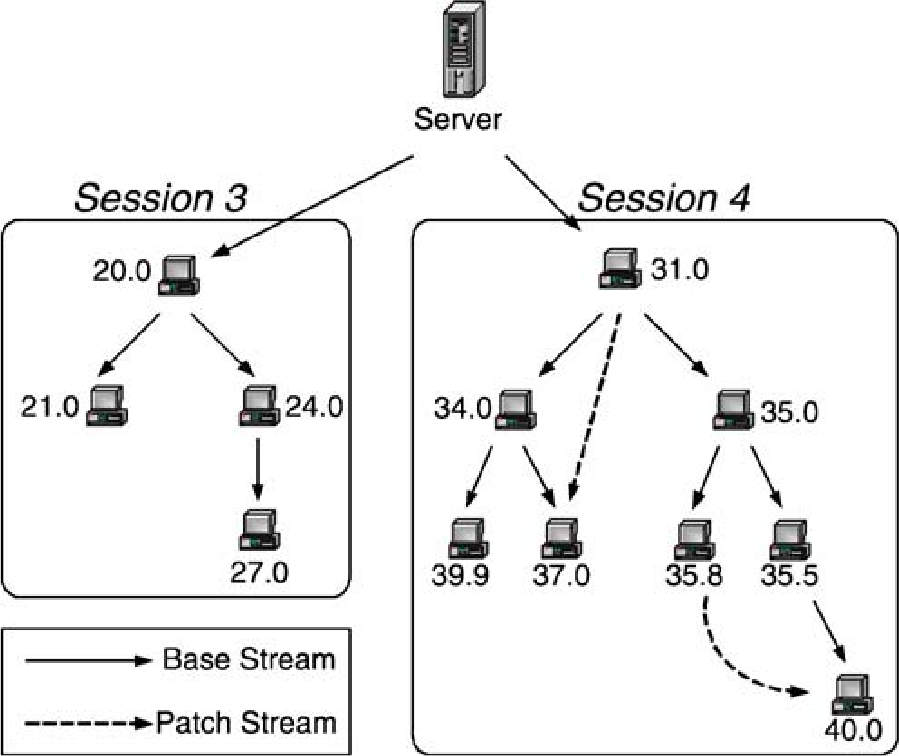
\includegraphics[width=0.5\textwidth]{src/img/p2p-systems/tree-based-vod}
  \caption{Tree-based Video-on-Demand}
  \label{fig:p2p-systems:tree-based-vod}
\end{figure}

In Figure~\ref{fig:p2p-systems:tree-based-vod}, there are two sessions (3 and 4) starting
at time 20.00 and
31.0, respectively, with a threshold of 10. Each user is maker with its
arrival time in the system. A straight arrow is used to represent a base
stream while a dotted arrow is a patch stream. Each user may receive
information from multiple users and it could also send information to multiple
users.

Mesh-based P2P file sharing network uses swarming (a collection of peers) and
is suitable for BitTorrent protocols. In a mesh-based network, peers connect
to other available peers depending on various factors such as availability,
bandwidth and protocol internals. Data delivery is highly similar to a
BitTorrent environment: there are seeders that possess all data and leechers
that possess only a subset of information. Data is fragmented into pieces and
is subsequently deliver (upon request) to various peers.

One of the first attempt to design a mesh-based P2P VoD service what
BiToS~\cite{bitos}. There are three components within the piece processing
activity in BiToS, as seen in Figure~\ref{fig:p2p-systems:bitos-vod}: the receive buffer, consisting of
all received information so far, the high priority set, consisting of pieces
that are required to allow smooth prerendering and the remaining set. The
optimal allocation of resources is an important design challenge.

\begin{figure}
  \centering
  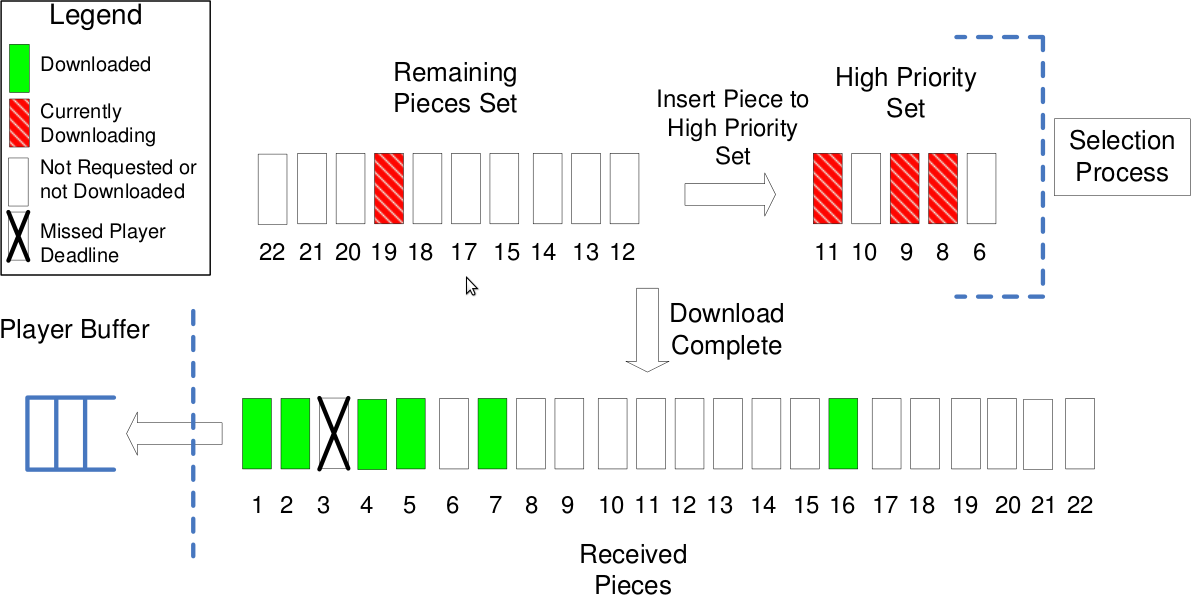
\includegraphics[width=0.7\textwidth]{src/img/p2p-systems/bitos-vod}
  \caption{Video-on-Demand in BiToS}
  \label{fig:p2p-systems:bitos-vod}
\end{figure}

\subsection{Live Streaming}
\label{subsec:p2p-systems:ls}

Live streaming consists of a server that is generating video content in real
time. Content dissemination is acted upon by other peers (clients). The video
playback is synchronized among all peers unlike peers in a VoD-like network,
where each peer may be positioned in a different part of the video.

Live streaming is usually making use of tree-based structures. A root server
is constantly (real-time) generating content and peers connect as clients
forming a tree. One of the basic frameworks for creating a tree-based overlay
is the deployment of IP level multicast. Due to implementation lack of
adoption, the IP level multicast hasn't been deployed and the multicast
function has been implemented at application level. A tree-based approach
could either be using a single tree streaming or multi-tree streaming.

In a single-tree streaming (Figure~\ref{fig:p2p-systems:single-tree-streaming}), a tree is
formed at application level based on the
root node which is equal to the server. Each user is a client and,
subsequently, a server and is joining the tree at a certain level. It receives
the live stream from the above node and delivers the information to the
children peers. A node receives data from a single parent node but may deliver
it to multiple nodes.

\begin{figure}
  \centering
  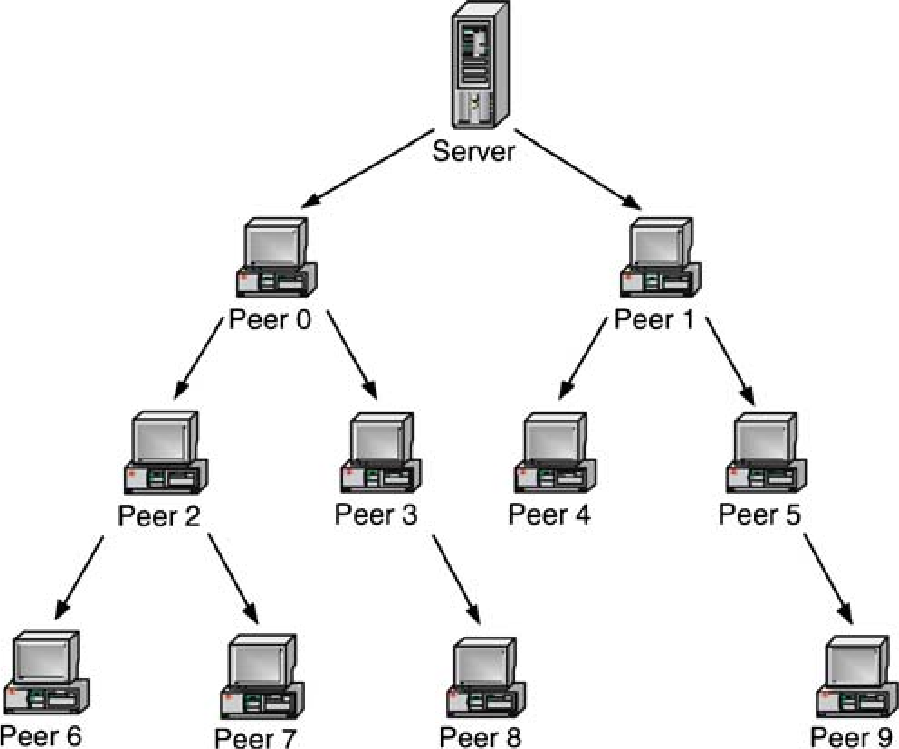
\includegraphics[width=0.5\textwidth]{src/img/p2p-systems/single-tree-streaming}
  \caption{Single-tree Streaming}
  \label{fig:p2p-systems:single-tree-streaming}
\end{figure}

An important issue of single-tree streaming is its construction. One would
required a small fan out and a small number of tree levels. A small fan out
would imply that nodes use their upload bandwidth to provide information to a
small number of nodes. A small number of levels means reduced delay in
propagating the streaming. As one can not achieve both a small number of
levels and a small fan out, compromise must be taken into account. Typically,
one would decide on the upload bandwidth available, compute the maximum fan
out and construct the tree accordingly. As more nodes are part of the network,
the number of levels would increase.

Another important issue is tree maintenance. Churning is an integral part of
a peer-to-peer network. Peers are dynamic and may leave the network (either
gracefully or unexpectedly). The child peers are not able to stream and the
tree has to be reconstructed as fast as possible. This is possible by
reassigning the peers to the server (similar to the arrival of a new peer).
The recovery may be done through the decision of a centralized server or in a
decentralized fashion.

The single-tree approach does possess important drawbacks. One of them is that
such a topology can not recover fast enough for frequent peer churn. Another
drawback is the lack of contribution from leaves. Leave peers don't put up use
of their upload bandwidth as no other peers are connected to them and request
streaming information.

The issue of leaf nodes is addressed through the use of multi-tree based
approaches. A server divides the streamed information in sub-streams. Each
peer joins all substreams, and information is flowed from the root node to
leaf nodes. A node may not (and usually is not satisfactory) be places in the
same position in each of the trees. In a given tree the node may be a leaf
node, meaning that it would only receive information from a substream; in
another substream it could be placed as an internal node. In the latter
substream the node would thus be able to use its upload bandwidth to provide
information to other peers. Multi-tree based systems would still suffer from
peer churning and tree maintenance has to be taken into account.

\subsection{Existing Solutions}
\label{subsec:p2p-systems:solutions}

Several commercial solutions have been developed around the concepts of
Peer-to-Peer streaming, making use of the scalability benefits and low cost
for distribution.

One of the most successful media streaming platforms,
Octoshape~\cite{octoshape},
uses various optimizations to deliver high quality streaming to users.
Octoshape was responsible for allowing the streaming of the US Inauguration of
President Barack Obama or the wedding of Prince William to Kate Middleton.
Octoshape uses a strategic partnership with different CDNs allowing a
distribution grid that minimizes cost but also ensure HD content availability
to average users. Its similar to a Peer-to-Peer engine that uses a plethora of
high quality peers to deliver content all over the world. Its optimizations
range from using a specialized Octoshape streaming protocol, multiple point
failover, loss resilience, a secure suite of multicast technologies.

While not a Peer-to-Peer streaming application, Akamai~\cite{akamai} is an
extended content delivery network that positions servers in various locations
to allow rapid access. Akamai created a globally distributed network of
tens of thousands of servers which is controlled by proprietary software.
Akamai servers typically mirror content which is subsequently server to users.
Akamai clients provide their content to Akamai servers which mirror and
distribute it across the Akamai network. Users would typically access the
server which is closest to their location.

Peer-to-Peer video streaming networks are PPTV and PPS.tv. Both are Chinese
oriented solutions. PPS.tv uses 8.9\% of the market share in China. Through
the use of P2P-streaming it supports high-volume traffic, allowing several
hundred users to watch a live stream at 300-500 Kbps with a server possessing
only 5-10 Mbps. PPTV offers both live streaming and video-on-demand, covering
a large specter of video assets for Chinese audience. Recently, the PPLive
team behind PPTV has migrated to a hybrid CDN-P2P cloud technology, called
PPCloud, considered as scalable and cost-effective. Several other solutions
have failed to gain momentum due to legal issues and locality constraints.

BitLet~\cite{bitlet}, an abbreviation for BitTorrent Applet is a BitTorrent
program enabling the use of the file sharing protocol inside a Java-enabled
web browser. The client download and uploads content as long as the program
window is open. As a specialized functionality, BitLet allows streaming audio;
it also possesses an experimental streaming video feature (based on Theora).

RTMFP~\cite{rtmfp} is a proprietary protocol developed by Adobe Systems that
enables direct Peer-to-Peer communication between multiple Adobe Flash Players
and applications build using Adobe AIR framework. RTMFP retains the benefits
of P2P-based streaming such as reduced bandwidth cost and scalability.
Cirrus~\cite{cirrus} is the technology that enables peer assisted networking
using RTMFP within the Adobe Flash platform. Cirrus 2, available in Flash
Player 10.1, supports groups, allowing application-level multicast and
reducing the load on the source publisher.

BitTorrent DNA (\textit{BitTorrent Delivery Network Accelerator}) is a program
designed to speed up viewing of streaming video through the use of the
BitTorrent protocol. BitTorrent DNA is UDP based, replacing regular TCP-based
bandwidth throttling with a much more sensitive technique. Users will be able
to download pieces of content from other users, releasing bandwidth pressure
from the original content source. It is targeted at streaming and online video
games.

O implementare ce se concentreaza in mod explicit pe distributia multimii
continutului divizat intr-o multitudine de parti este ceea ce numim Swarmcast.
Se bazeaza pe puterea serverului central de a administra o retea cu clienti
distribuiti.

Swarmcast este promovat ca un sistem de distributie de continut de mare viteza
pentru fisierele mari în locul unui sistem cu distributie de fisiere. Editorii
fisierelor cu continut foarte mare, cu multe solicitari asteptate, pot sa
distribuie eficient si fiabil aceste fisiere multor utilizatori cu costuri
mici pentru latimea de banda. Utilizatorii obseva ca pot descarca fisiere mari
repede si mai fiabil pentru ca tehnologia de swarming se adapteaza cererilor
privind alocarea spatiului de scara si mutiplicarea continutului aproape de
punctele de cerere.

Solutia oferită de Swarmcast are doua componente principale:

\begin{itemize}
  \item{Swarmcast Gateway este o parte comerciala a programului serverului.Ca
  efect, publica continutul ca parti unui număr de noduri si apoi distribuie
  fiecare cerere de descarcare primita de la utilizator catre nodurile
  disponibile sa serveasca aproape toate partile fisierului cerut.}
  \item{Swarmcast Client este programul pe care un utilizator poate sa il
  descarce gratuit. Il instaleaza pe propria masina pentru activarea
  descarcarii fisierelor swarmcast.}
\end{itemize}

Tehnologia poate fi facuta sa lucreze si cu alte aplicatii, cum ar fi manageri
de descarcare, software updaters si cu aplicatii de distributie de fisiere.

Swarmcast se bazeaza pe modul in care clientii de Web solicita fisiere de la
un server HTTP Web. Ofera o arhitectura centrată pe conținut, unde continutul
in mod original este publicat si apartine serverului central. Fiecarui fisier
i se aloca o cheie (hashed-key SHA-1), care asigura integritatea datelor si
independenta numelui si permite autentificarea si functionalitati private.

Cerintele pentru un transfer al datelor rapid si fiabil catre multi
utilizatori sunt indreptate in doua directii: oferind multe cai P2P pentru a
reduce banda pe fiecare cale, si o codare redundanta avansata a partilor
transferate. Se incearca in mod agresiv impingerea continutului catre retelele
locale de perechi interesate, eliberand banda centrala si minimizand caile de
date pentru majoritatea nodurilor. Tehnologia Swarmcast in implementarea sa de
baza nu mentine o retea P2P durabila. In schimb presupune un server central
normal ca ultima sursa pentru intregul continut. Utilizatorii stiu doar de
aceasta sursa centrala, si poate fi in locuri diferite, sau poate reflectata
in moduri traditionale.

Utilizatorii parcurg si cer anumite fisiere prin intermediul clientilor
acestora, care se conecteaza la server prin gateway pentru a descarca
fisierele. Apoi serverul central permite descarcarea. Fisierul este impartit
apoi in pachete codate indentificabile de gateway si trimise clientilor.
Cerintele unui anumit fisier nu sunt cu mult diferite fata de descarcarile
client-server normale.

\subsection{Legal Aspects}
\label{subsec:p2p-streaming-legal}

Apart from the technical challenges surrounding a Peer-to-Peer based solution,
issues are constantly in place regarding legal aspects of data distribution.
As most of the content is owned by publishing houses, even tens of years after
its creation, it's implied transferring much of that content is illegal. A
typical BitTorrent network doesn't integrated features such as encryption, DRM
and ownership information, meaning that it is highly plausible that, by acting
to download a piece of content, you come across a legal aspect. Often vague
and inconsistent legislation only adds to the problem. The plethora of legal
issues concerning BitTorrent is made apparent by the high number of legal
disputes regarding various distribution sites, one of the most famous being
``The Pirate Bay''~\cite{pirate-bay}. Various Peer-to-Peer streaming solutions have
failed to gain momentum or have even been closed/disabled due to legal
troubles.

The legal aspects of Peer-to-Peer streaming solutions incur a greater
difficulty in providing a successful business model. There are two approaches.

A first approach is one that considers using a proprietary and secure platform
that selectively transfers information to users, possibly in an encrypted
form, such that other users in the swarm may not access that information. This
approach would be adequate to large media creators that want to deliver their
content to users but want to keep information private and only paying users
would access that -- as it is typical in CDN-based solutions such as Akamai.

The second solution takes into account that protecting content ownership and
making profit out of it is not a priority. Rather making profit from side
activities such as commercials, user credits, premium content, social
networking solutions. This model is close to the functionality provided by
YouTube where all content is available, a user may choose to ingest content
and profit is taken out of commercials. The selective insertion of commercials
into video streams is a possible solution for making profit out of ``free''
content into Peer-to-Peer networks.

There are still lingering questions regarding the possibility of success for
any of the above solutions. Given the vague legislation and continuous debates
between anti and pro-piracy groups, a suitable solution is yet to come out.

\section{BitTorrent}
\label{sec:p2p-systems:bittorrent}

One of the disadvantages of P2P systems is the ``opening'' for \textit{free
riding} \cite{free-riding} or \textit{free loading}. While peer are generally
considered to be altruistic, this behavior is not generally enforced. Free
riding is equivalent to an egoistic behavior, where a peer gets information
from other peers and gives nothing back. This behavior disables the very
nature of P2P systems: sharing information.

If a given network consists of a high number of free riders, then data load
among peer is unbalanced. When a new node share a popular file in the native
P2P system, it will attract a large number of connection. In case of free
riding, this node has to use more bandwidth for more clients.

O analiză întreprinsă de cercetătorii de la Xerox Palo Alto Research Center
indică faptul că circa 50\% dintre fișierele partajate sunt stocate pe 1\%
dintre noduri. Circa 70\% din utilizatorii Gnutella nu partajează fișiere cu
alți utilizatori. Cu alte cuvinte, ei doar "descarcă" resurse și sunt denumiți
"freeloaders" sau "freeriders".

BitTorrent is a new protocol being used to solve the free riding problem,
though not completely \cite{free-riding}. The idea behind the protocol is
fairly simple: the node that plays the role of the server breaks the file in
pieces. If the file is requested by more clients simultaneously, each client
will get a different piece of that file. When a client gets a complete piece
it will allow other clients to download that subfile, while it will continue
downloading the second piece. In other words, the node acts simultaneously as
a client and a server after receiving the first piece. The process continues
until the download completes.

The BitTorrent protocol is highly suitable for downloading large files where
the download process takes a long time. As a direct consequence, more
``server'' peers are available for a longer duration. More clients will not
result in a performance decrease of the whole network as the load is
distributed.

Figure~\ref{fig:p2p-systems:bittorrent-sharing} se prezintă o diagramă
schematică.  Serverul are 4 subfișiere. Fiecare client obține un subfișier de
la server la un moment dat.  După cum se observă, clientul 1 obține aceste 4
subfișiere de la sisteme de calcul diferite. Modul în care subfișierele ajung
la client pot să nu respecte ordinea inițială. Algoritmul BitTorrent va
încerca maximizarea numărului de subfișiere disponibile pentru download la un
moment dat.

\begin{figure}
  \centering
  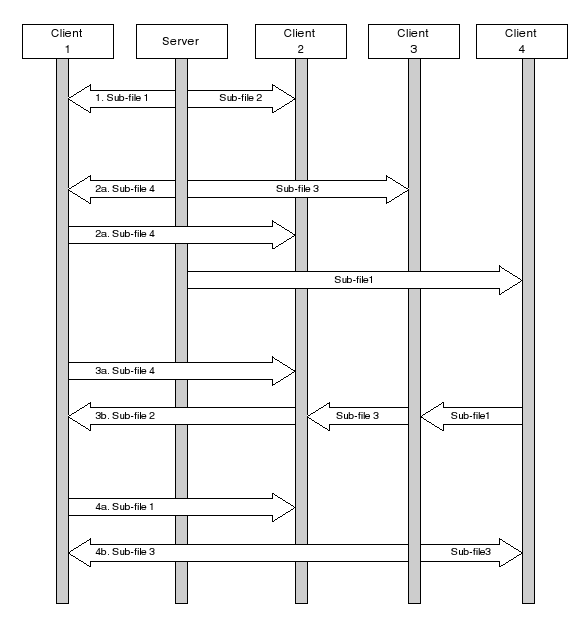
\includegraphics[width=0.4\textwidth]{src/img/p2p-systems/bittorrent-sharing}
  \caption{BitTorrent File Sharing}
  \label{fig:p2p-systems:bittorrent-sharing}
\end{figure}

Pentru a descărca un fișier un utilizator folosește următorii pași:

\begin{itemize}
  \item instalează o aplicație BitTorrent
  \item navighează Web-ul
  \item găsește un fișier pe un server
  \item selectează locația unde să fie salvat fișierul
  \item așteaptă încheierea procesului
  \item instruiește programul să se închidă (procesul de upload continuă până
  când utilizatorul realizează acest pas)
\end{itemize}

\subsection{BitTorrent Keywords}

A \textit{peer} is the basic unit of action in any P2P system, and, as such, a
BitTorrent system. It is typically a computer system or program that is
actively participating in sharing a given file in a P2P network. A peer is
generally characterized by its implementation, download/upload bandwidth
capacity (or limitation), download/upload speed, number of download/upload
slots, geolocation and general behavior (aggressiveness, entry--exit time
interval, churn rate).

The context in which a BitTorrent content distribution session takes place is
defined by a BitTorrent \textbf{swarm} which is the peer ensemble that
participate in sharing a given file. It is characterized by the number of
peers, number of seeders, file size, peers' upload/download speed. A healthy
swarm, one that allows rapid content distribution to peers, is generally
defined by a good proportion of seeders and stable peers (peers that are part
of the swarm for prolonged periods of time).

A swarm consists of two types of peers: leechers and seeders. A
\textbf{seeder} is a peer that has complete access to the distributed content
and is, thus, only uploading data. A \textbf{leecher} has incomplete access to
distributed content and is both uploading and downloading. The BitTorrent
negotiation protocol uses a form of tit-for-tat that forces peers to upload in
order to download (though this has been proven to be abused
\cite{free-riding}) therefore ensuring fairness and rapid distribution. A good
number of healthy seeders is a requirement for healthy swarms that allow rapid
distribution of data.

A swarm is given birth by an \textit{initial seeder} which is the peer sharing
a file it has complete access to. The seeding/sharing process within a swarm
is started through a metafile, a \textbf{.torrent} file, that defines swarm
trackers and piece hashes to ensure content integrity. Typically, a peer uses
a web server to download a .torrent file and then uses a BitTorrent client to
interpret it and take part into a swarm. It is possible to create different
swarms for the same content by using different trackers in a .torrent file.

Communication of peers in a swarm is typically mediated by a BitTorrent
\textbf{tracker} or several trackers which are defined in the .torrent file.
It is periodically contacted by the peers to provide information regarding
piece distribution within the swarm. A peer would receive a list of peers from
the tracker and then connect to these peers in a decentralized manner. As it
uses a centralized tracker, the swarm may suffer if the tracker is
inaccessible or crashes. Several solutions have been devised, such as PEX
(Peer EXchange) \cite{pex} or DHT (Distributed Hash Table) \cite{dht-paper}.

\todo{add architecture}

\subsection{BitTorrent Internals}

The core of the BitTorrent protocol is the \textit{tit for tat} mechanism,
also called \textit{optimistic unchoking} allowing for upload bandwidth to be
exchanged for download bandwidth. A peer is hoping another peer will provide
data, but in case this peer doesn't upload, it will be \textit{choked}.
Another important mechanism for BitTorrent is \textit{rarest piece first}
allowing rapid distribution of content across peers. If a piece of the content
is owned by a small group of peers it will be rapidly requested in order to
increase its availability and, thus, the overall swarm speed and performance.

\todo{more on this}

\section{Issues and Challenges in Peer-to-Peer Systems}
\label{sec:p2p-systems:issues}

\todo{issues}

%Viitorul rețelelor P2P
%
%Tehnologia de tip P2P promite să ofere fiecărui individ acces la servicii și
%conținut distribuit liber. Termenul liber nu înseamnă neapărat fără cost,
%fiind disponibile mai multe metode de plată în practică. Posesia individuală
%a conținutului și serviciilor înseamnă acces personal direct, libertate în
%utilizare și libertate în mișcare. La fel ca și în cazul posesiei de
%proprietate fizică, presupunerea este că individul poate delega drepturi
%suplimentare entităților în care are încredere.
%
%Viziunea P2P încapsulează, de asemenea, conceptul împuternicirii
%utilizatorului, care este o ambiție importantă de multe ori pierdută sub
%deviza "ușurinței în utilizare".
%
%Câteva dintre expresiile împuternicirii utilizatorului sunt aceste acțiuni:
%crearea de conținut și servicii și posibilitatea localizării lor pe orice
%dispozitiv disponibil
%accesarea resurselor și serviciilor cu orice dispozitiv disponibil indiferent
%de sursă, locație sau timp
%gestionarea propriului conținut și a serviciilor
%partajarea de conținut cu familia, cunoscuții și restul lumii
%menținerea confidențialității și integrității informațiilor personale și
%proprietare
%coordonarea livrării de servicii și conținut
%personalizarea prezentării, conținutului și serviciilor
%
%Internet2
%
%Internet2 este format în jurul unui consorțiu de 180 de universități care
%lucrează în parteneriat cu guvernul și industria și a fost fondat pentru
%dezvoltarea și utilizarea tehnologiilor și aplicațiilor de rețea avansate.
%Așa cum se menționează și pe site-ul web (http://www.internet2.edu) deviza
%este "accelerarea creării Internet-ului de mâine". Tehnologiile peer sunt un
%motiv des întâlnit în efortul Internet2.
%
%Motivația din spatele consorțiului este că cercetările universitare au nevoie
%crescândă de colaborarea personalului și hardware-ului localizat în campusuri
%aflate de-a lungul țărilor în moduri care nu sunt posibile cu infrastructura
%Internet-ului de astăzi. Cererea mare de lățime de bandă a fost o motivație
%inițială. Mai mult, universitățile sunt principala sursă de cerere de
%tehnologii avansate și talentul necesar pentru implementarea lor.
%
%Pe scurt, Internet2 intenționează crearea unei rețele distribuite de servicii
%care să maximizeze utilizarea resurselor de Internet. Un concept introdus
%este acela al canalelor sau colecțiilor de conținut care sunt văzute ca un
%superset a ceea ce poate accesa Web-ul astăzi. Este o agregare a diverselor
%forme de conținut colectate în mod deliberat și furnizate utilizatorilor. Un
%exemplu ar putea fi întregul ansamblu de conținut digital folosit în timpul
%unui curs conținând documente, video, software, seturi de date, simulări,
%examene online etc.
%
%Internet2 nu este intenționat să înlocuiască Internet-ul tradițional. Este
%proiectat să lucreze în paralel pentru deservirea constituenților
%particulari. Destul de probabil, Internet2 se va afla tot timpul pe vârful
%tehnologic. Mare parte din tehnologia dezvoltată pentru Internet2 va fi mai
%mult ca sigur folosită peste Internet-ul original.
%
%P2P-Next
%
%P2P-Next urmărește contruirea următoarei generații de platforme P2P de
%librare de conținut. Proiectarea, dezvoltarea șî lansarea aplicațiilor se
%realizează de un consorțiu format din membri academici și industriali.
%
%Ideea din spatele P2P-next este posibilitatea ca tehnologiile peer pot
%furniza conținut profesional și creat de utilizator într-un mod cât mai
%eficient și cu costuri reduse esențial pentru viitorul competitiv al
%Internet-ului. P2P-Next urmărește facilitarea a noi scenarii de afaceri spre
%o platformă centrată pe utilizator independentă de timp și loc. Crearea unei
%platforme de dezvoltare permite aplicații modulare, integrarea aplicațiilor,
%reutilizarea codului. Aceasta se traduce într-o dezvoltare rapidă a
%aplicațiilor de livrare de conținut care valorifică serviciile și conținutul
%furnizorilor asociați.
%
%P2P-Next urmărește dezvoltarea unei platforme open-source și open-standard.
%Se urmărește obținerea de avansuri în mai multe domenii incluzând distribuția
%de conținut, acces facil la conținut larg de informații, social networking,
%idei de afaceri pentru publicitate. Suma acestor avansuri se dorește a fi un
%pas în mutarea accesului la informație din mâna producătorilor în mâinile
%consumatorilor și permițând consumtatorilor utilizarea resurselor de conținut
%de oriunde și oricând.
%
%Bibliografie
%
%[1] Andy Oram - Peer-to-Peer: Harnessing the Power of Disruptive Technologies, O'Reilly & Associates, Feb 2001
%[2] Ramesh Subramanian, Bran Goodman - Peer-to-Peer Computing: The Evolution of a Disruptive Technology, Idea Group Inc., 2005
%[3] Bo Leuf - Peer to Peer: Collaboration and Sharing over the Internet, Addison Wesley, 2002
%[4] Dreamtech Software Team - Peer-to-Peer Application Development, Hungry Minds, 2002
%[5] Alfred Wai-Sing Loo - Peer-to-Peer Computing: Building Supercomputers with Web Technology, Springer, 2007
%[6] Yoram Kullbak, Danny Bickson – The eMule Protocol Specification, 2005
